\documentclass{IFES-beamer}
\usepackage{pgfplots}
\pgfplotsset{compat=1.15}
\usepackage{amssymb}
\usepackage{graphicx,xcolor}
\usepackage{color}
\definecolor{ccqqqq}{rgb}{1,0,0}
\definecolor{darkGreen}{rgb}{0,.5,0}


%%%%%%%%%%%%%%%%%%%%%%%%%%%%%%%%%%%%
%  Defini o estlo no algorithmic
%%%%%%%%%%%%%%%%%%%%%%%%%%%%%%%%%%%%%
\newcommand{\red}{\color{red}}
\newcommand{\green}{\color{green}}
\newcommand{\TODO}[1]{{{\red #1}}}
\newcommand{\var}[1]{$#1$} %define estilo de nomes de variaveis
\newcommand{\defi}[1]{\textbf{#1}} % defini estilo ao definir algo no texto
\def\Nil{\text{NIL}}

\newcommand\circledmark{%
  \ooalign{%
    \hidewidth
    \kern-0.4ex\raisebox{-2.1ex}{\scalebox{5.5}{\textcolor{darkGreen}{\textbullet}}}
    \hidewidth\cr
    \kern-.6ex\raisebox{.6ex}{\color{white}$\checkmark$}\cr
  }%
}
\newcommand\custommark{%
  \ooalign{%
    \hidewidth
    \kern-0.4ex\raisebox{-2.1ex}{\scalebox{5.5}{\textcolor{white}{\textbullet}}}
    \hidewidth\cr
    \kern-.6ex{\color{black}$\checkmark$}\cr
  }%
}


\usepackage[Algoritmo]{algorithm}
\usepackage[noend]{algpseudocode}
\algrenewcommand\algorithmicif{\textbf{se}}
\algrenewcommand\algorithmicfor{\textbf{para}}
\algrenewcommand\algorithmicelse{\textbf{senão}}
\algrenewcommand\algorithmicwhile{\textbf{enquanto}}
\algrenewcommand\algorithmicdo{\textbf{faça}}
\algrenewcommand\algorithmicend{\textbf{fim}}
\algrenewcommand\algorithmicthen{\textbf{então}}
\algrenewcommand\algorithmicreturn{\textbf{retorne}}



\newcommand{\AlgoName}[1]{\text{\scshape #1}}

%%%%%%%%%%%%%%%%%%%%%%%%%%%%%%%%%%%%%
% Comandos de notação assintotica   %
%%%%%%%%%%%%%%%%%%%%%%%%%%%%%%%%%%%%%
\renewcommand{\O}[1]{\text{O}(#1)}
\newcommand{\OTheta}[1]{\Theta(#1)}

%%%%%%%%%%%%%%%%%%%%%%%%%%%%%%
%    Nomes de váriaveis      %
%%%%%%%%%%%%%%%%%%%%%%%%%%%%%%
\newcommand{\varname}[1]{\textit{#1}}
\newcommand{\altvarname}[1]{$#1$}
\newcommand{\node}{\mathit{n\acute{o}}}
%\newcommand{\var}{\mathit{var}}

%%%%%%%%%%%%%%%%%%%%%%%%%%%%%%
%     Métodos de Grafos      %
%%%%%%%%%%%%%%%%%%%%%%%%%%%%%%
\newcommand{\graphCreate}{\AlgoName{novoGrafo}}
\newcommand{\graphAdd}{\AlgoName{ligueGLA}}
\newcommand{\graphDel}{\AlgoName{removaGLA}}

%%%%%%%%%%%%%%%%%%%%%%%%%%%%%%
%     Métodos de Treap       %
%%%%%%%%%%%%%%%%%%%%%%%%%%%%%%
\newcommand{\treapCreate}{\AlgoName{novoNó}}
\newcommand{\treapSearch}{\AlgoName{busca}}
\newcommand{\treapGetLast}{\AlgoName{último}}
\newcommand{\treapGetRoot}{\AlgoName{raiz}}
\newcommand{\treapOrder}{\AlgoName{ordem}}
\newcommand{\treapJoin}{\AlgoName{junta}}
\newcommand{\treapSplit}{\AlgoName{corta}}
\newcommand{\treapSplitRight}{\AlgoName{cortaDireita}}
\newcommand{\treapGetSize}{\AlgoName{tamanho}}
\newcommand{\treapGetEdgesLevel}{\AlgoName{arestasDeNível}}

\newcommand{\treapFirst}{\AlgoName{primeiro}}
\newcommand{\treapLast}{\AlgoName{último}}
\newcommand{\treapPredecessor}{\AlgoName{\AlgoName{Pred}}}    %(F, u, v)

%%%%%%%%%%%%%%%%%%%%%%%%%%%%%%
% Métodos de Euler Tour Tree %
%%%%%%%%%%%%%%%%%%%%%%%%%%%%%%
\newcommand{\ETTCreate}{\AlgoName{novoETT}}     % (v)
\newcommand{\ETTAddEdge}{\AlgoName{ligueETT}} % ($F$, $uu$, $vv$)
\newcommand{\ETTDelEdge}{\AlgoName{removaETT}} % ($F$, $uu$, $vv$)
\newcommand{\ETTQuery}{\AlgoName{conectadoETT}} % ($F$, $uu$, $vv$)
\newcommand{\ETmovetofront}{\AlgoName{movaInício}} % ($F$, $uu$)


%%%%%%%%%%%%%%%%%%%%%%%%%%%%%%%%%%
% Métodos da tabela hash         %
%%%%%%%%%%%%%%%%%%%%%%%%%%%%%%%%%%
\newcommand{\dymForestHash}{$H$}  %simbolo que identifica a matriz/hash da floresta
\newcommand{\nivel}{\AlgoName{nível}} 
\newcommand{\hashCreate}{\AlgoName{novoDicio}}     

%%%%%%%%%%%%%%%%%%%%%%%%%%%%%%%%%%
% Métodos de Florestas dinamicas %
%%%%%%%%%%%%%%%%%%%%%%%%%%%%%%%%%%
\newcommand{\dymForestCreate}{\AlgoName{novaFD}}  %(n)
\newcommand{\dymForestAddEdge}{\AlgoName{ligueFD}}    %(F, u, v)
\newcommand{\dymForestDelEdge}{\AlgoName{removaFD}}    %(F, u, v)
\newcommand{\dymForestQuery}{\AlgoName{\AlgoName{conectadoFD}}}    %(F, u, v)

%%%%%%%%%%%%%%%%%%%%%%%%%%%%%%%%%%
% Métodos de Grafos dinamicas %
%%%%%%%%%%%%%%%%%%%%%%%%%%%%%%%%%%
\newcommand{\dymGraphCreate}{\AlgoName{novoGD}}    %(n)
\newcommand{\dymGraphAddEdge}{\AlgoName{ligueGD}} %(G, u, v)
\newcommand{\dymGraphDelEdge}{\AlgoName{removaGD}} %(G, u, v)
\newcommand{\dymGraphQuery}{\AlgoName{\AlgoName{conectadoGD}}} %(G, u, v)
\newcommand{\dymGraphReplace}{\AlgoName{\AlgoName{substituaGD}}} %(G, u, v, i)
\newcommand{\dymGraphHash}{$H$}  %simbolo que identifica a matriz/hash da floresta

%%%%%%%%%%%%%%%%%%%%%%%%%%%%%%
% Métodos de Link/Cut Tree   %
%%%%%%%%%%%%%%%%%%%%%%%%%%%%%%

\newcommand{\linkcutCreate}{\AlgoName{newLCT}}
\newcommand{\linkcutDestroy}{\AlgoName{delLCT}}
\newcommand{\linkcutAddEdge}{\AlgoName{link}}    %(F, u, v)
\newcommand{\linkcutDelEdge}{\AlgoName{cut}}    %(F, u, v)
\newcommand{\linkcutEvert}{\AlgoName{\AlgoName{evert}}}    %(v)
\newcommand{\linkcutMax}{\AlgoName{\AlgoName{max}}}    %(F, u, v)
\newcommand{\linkcutMin}{\AlgoName{\AlgoName{min}}}    %(F, u, v)
\newcommand{\linkcutParent}{\AlgoName{\AlgoName{parent}}}    %(F, u, v)
\newcommand{\linkcutQuery}{\AlgoName{\AlgoName{conectadoLC}}}    %(F, u, v)
\newcommand{\linkcutWeight}{\AlgoName{\AlgoName{set weight}}}    %(F, u, v)
\newcommand{\linkcutRoot}{\AlgoName{\AlgoName{get Root}}}    %(F, u, v)

%%%%%%%%%%%%%%%%%%%%%%%%%%%%%%%%%%%%%%%
% Métodos de Link/Cut Tree com ordem  %
%%%%%%%%%%%%%%%%%%%%%%%%%%%%%%%%%%%%%%%

\newcommand{\LCOMakeOcto}{\AlgoName{Create Octo}}
\newcommand{\LCODestroyOcto}{\AlgoName{Destroy Octo}}

\newcommand{\LCOMakeNode}{\AlgoName{Make edge}}
\newcommand{\LCODestroyNode}{\AlgoName{Make edge}}
\newcommand{\LCOLink}{\AlgoName{Link}}
\newcommand{\LCOMerge}{\AlgoName{Merge}}
\newcommand{\LCOSplit}{\AlgoName{Split}}
\newcommand{\LCOCycle}{\AlgoName{Cycle}}
\newcommand{\LCOParent}{\AlgoName{\AlgoName{Parent}}}    %(F, u, v)
\newcommand{\LCORoot}{\AlgoName{Root}}
\newcommand{\LCOAddCost}{\AlgoName{Set weight}}
\newcommand{\LCOMax}{\AlgoName{\AlgoName{Find max}}}    %(F, u, v)
\newcommand{\LCOMin}{\AlgoName{\AlgoName{Find min}}}    %(F, u, v)
\newcommand{\LCOEvert}{\AlgoName{\AlgoName{Evert}}}    %(F, u, v)
\newcommand{\LCOConnected}{\AlgoName{\AlgoName{Connected}}}    %(F, u, v)
\newcommand{\LCOFindNode}{\AlgoName{Find node}}

%%%%%%%%%%%%%%%%%%%%%%%%%%%%%%
%     Métodos de MSF         %
%%%%%%%%%%%%%%%%%%%%%%%%%%%%%%
\newcommand{\MSFCreate}{\AlgoName{novoGDP}} %(n)
\newcommand{\MSFupdate}{\AlgoName{mudaPesoGDP}} %(n)
\newcommand{\MSFaddEdge}{\AlgoName{ligueGDP}}    %(G, u, v, w)
\newcommand{\MSFdelEdge}{\AlgoName{removaGDP}}    %(G, u, v)
\newcommand{\MSFweight}{\AlgoName{pesoGDP}}    %(G)

\newcommand{\dymGraphReplaceMSF}{\AlgoName{substituaGDP}} %(G, u, v, i)
\newcommand{\treapGetEdgeMinWeight}{\AlgoName{arestaMinPesoGDP}}


%%%%%%%%%%%%%%%%%%%%%%%%%%%%%%
%     Métodos de VPSP
% Verify partial sum of permutations%
%%%%%%%%%%%%%%%%%%%%%%%%%%%%%%

\newcommand{\VPSPconvert}{\AlgoName{converta}}
\newcommand{\VPSPupdate}{\AlgoName{substitua}}
\newcommand{\VPSPverify}{\AlgoName{verifique}}




% --------------------------------------------------- %
%                  Presentation info	              %
% --------------------------------------------------- %
\title[Algorit. em conexidade dinâmica]{Algoritmos para conexidade em grafos dinâmicos}
%\subtitle{Subtitle}
\author[Arthur Rodrigues]{Arthur Henrique Dias Rodrigues\\{\footnotesize sob orientação de}\\Cristina Gomes Fernandes}
\institute[IME-USP]{
  Instituto de Matemática e Estatistica\\
  USP
}
\day=22
\month=11
\year=2024
\subject{Algorit. em conexidade dinâmica} % metadata

% --------------------------------------------------- %
%                    Title + Schedule                 %
% --------------------------------------------------- %


\begin{document}
\begin{frame}
  \titlepage
\end{frame}

\begin{frame}{Sumário}
  \tableofcontents
\end{frame}

% --------------------------------------------------- %
%                      Presentation                   %
% --------------------------------------------------- %

\section{Problemas}
\subsection{Definições}
\begin{frame}{Problema de conexidade dinâmicas}
\begin{block}{Contexto}
\begin{itemize}
    \item $G$: grafo;
    \item $n$: número de vértices em~$G$;
    \item $F$: floresta;
    \item $u$,$v$: vértices.
    \end{itemize}
\end{block}

\begin{exampleblock}{Problema de conexidade dinâmicas}
\begin{itemize}
\item \dymGraphCreate($n$): retorna um grafo dinâmico com $n$ vértices isolados;
\item \dymGraphAddEdge($G$, $u$, $v$): adiciona aresta $uv$ a~$G$;
\item \dymGraphDelEdge($G$, $u$, $v$): remove $uv$ de $G$; e
\item \dymGraphQuery($G$, $u$, $v$): retorna verdadeiro se $u$ e~$v$ estão na mesma componente conexa de~$G$ e falso, caso contrário.
\end{itemize}
\end{exampleblock}
\end{frame}

\begin{frame}{Problemas MSF}
\boxblue{MSF: floresta maximal de peso mínimo}
\begin{block}{Grafo ponderado}
Cada aresta possui um peso associado.
\end{block}

\begin{exampleblock}{Problema da floresta maximal de peso mínimo em grafos ponderados dinâmicos}
\begin{itemize}
\item \MSFCreate($n$): devolve um grafo ponderado com $n$ vértices isolados;
\item \MSFaddEdge($G$,$u$,$v$,$w$): adiciona a aresta~$uv$ com peso~$w$ em~$G$;
\item \MSFdelEdge($G$,$u$,$v$): remove a aresta $uv$ de $G$; e
\item \MSFweight($G$): devolve o peso de uma MSF de $G$.
\end{itemize}
\end{exampleblock}
\end{frame}

\subsection{Resultados conhecidos}
\begin{frame}{Resultados conhecidos}
\begin{alertblock}{Limitante inferior (Patrascu e Demaine)~\cite{lowerBoundPatrascu}, 2006}
Todo algoritmo que resolve os problemas de conexidade dinâmica e de MSF dinâmica possuem consumo de tempo~$\Omega(\lg n)$.
\end{alertblock}
\begin{block}{Conexidade dinâmicas~(Holm et al.~\cite{poly_log}, 2001)}
Para árvores,~$\O{\lg n}$;\\
Grafos gerais,~$\O{\lg^2 n}$ amortizado.
\end{block}

\begin{block}{MSF~(Holm et al.~\cite{poly_log}, 2001)}
Para grafos gerais, amortizado~$\O{\lg^4 n}$.
\end{block}
\end{frame}

\begin{frame}{Resultados conhecidos}
\begin{block}{Kapron et al. (2013)~\cite{bruceM}}
    $\O{\lg^5 n}$ no pior dos casos, mas que pode haver falso positivo na consulta; 
\end{block}
\begin{block}{Chen et al. (2022)~\cite{QC22}}
    Apresenta bom desempenho prático, mas...
    \begin{itemize}
        \item os autores não apresentam análise de complexidade;
        \item não compara com a solução de Holm et al.~\cite{poly_log} ou Kapron et al.~\cite{bruceM}.
    \end{itemize}
\end{block}
\pause
\begin{block}{Implementações conhecidas de Holm et al.}
\begin{itemize}
    \item Gabriel Russo~\cite{russo}, em C++;
    \item Raj Iyer, David Karger, Hariharan Rahul e Mikkel Thorup~\cite{EmpiricalStudy2002} em C.
\end{itemize}
\end{block}
\end{frame}

\section{Conexidade em florestas dinâmicas}
\subsection{Definição}
\begin{frame}{Conexidade em florestas dinâmicas}

\begin{exampleblock}{Problema de conexidade em florestas dinâmicas}
\begin{itemize}
\item \dymForestCreate($n$): retorna uma floresta dinâmica com $n$ vértices isolados;
\item \dymForestAddEdge($F$,$u$,$v$): adiciona $uv$ a~$F$;
\item \dymForestDelEdge($F$,$u$,$v$): remove $uv$ de $F$; e
\item \dymForestQuery($F$,$u$,$v$): retorna verdadeiro se $u$ e~$v$ estão na mesma componente conexa de~$F$ e falso, caso contrário.
\end{itemize}
\end{exampleblock}
\end{frame}

\subsection{Euler Tour Trees}

\begin{frame}{Sequência Euleriana}
\begin{center}
\begin{figure}
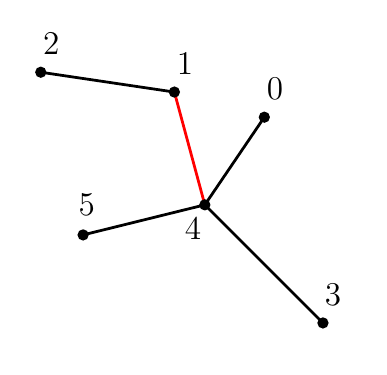
\begin{tikzpicture}[dot/.style={draw,circle,fill,inner sep=1.5pt},line width=1pt,x=1.5cm,y=1.5cm]
\clip(.5,.8) rectangle (3.3,3.5);
\draw [line width=1pt] (1.7420645075484014,2.9548225063123694)-- (0.6109449986613309,3.1228105521866865);
\draw [line width=1pt,color=ccqqqq] (1.7420645075484014,2.9548225063123694)-- (2,2);
\draw [line width=1pt] (2,2)-- (0.9693194965265414,1.7453085760172875);
\draw [line width=1pt] (2,2)-- (3,1);
\draw [line width=1pt] (2,2)-- (2.5036103155119798,2.742037648204901);
\begin{scriptsize}
\draw [fill=black,bend left] (1.7420645075484014,2.9548225063123694) circle (1.5pt);
\draw[color=black] (1.8316581320147085,3.195605372065557) node {{\large 1}};
\draw [fill=black] (0.6109449986613309,3.1228105521866865) circle (1.5pt);
\draw[color=black] (0.7005386231276353,3.363593417939874) node {{\large 2}};
\draw [fill=black] (2,2) circle (1.5pt);
\draw[color=black] (1.9,1.8) node {{\large 4}};
\draw [fill=black] (0.9693194965265414,1.7453085760172875) circle (1.5pt);
\draw[color=black] (1,2) node {{\large 5}};
\draw [fill=black] (3,1) circle (1.5pt);
\draw[color=black] (3.0859688745429477,1.2357448368651927) node {{\large 3}};
\draw [fill=black] (2.5036103155119798,2.742037648204901) circle (1.5pt);
\draw[color=black] (2.5932039399782822,2.9828205139580892) node {{\large 0}};
\end{scriptsize}
\end{tikzpicture}
%\documentclass[border=5pt,tikz]{standalone}
%\usetikzlibrary{positioning}
%\begin{document}
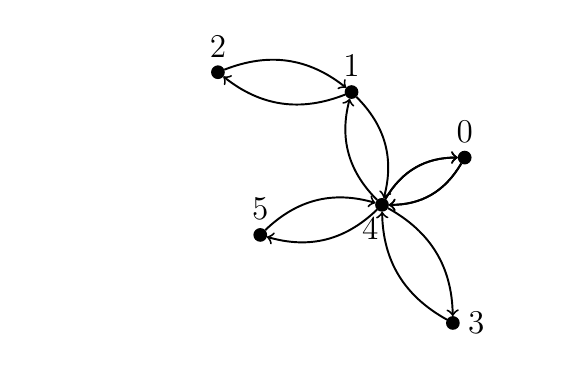
\begin{tikzpicture}[dot/.style={draw,circle,fill,inner sep=1.5pt},line width=.7pt,x=1.5cm,y=1.5cm]
\clip(-1,.8) rectangle (3.3,3.5);
\begin{scriptsize}
\node[label=above:{\large 0}] (r0) at (2.7,2.4) [dot] {};

\node[label=above:{\large 1}] (r1) at (1.7420645075484014,2.9548225063123694) [dot] {};
%\draw[color=black] (1.8316581320147085,3.195605372065557) node {$1$};


\node[label=above:{\large 2}] (r2) at (0.6109449986613309,3.1228105521866865) [dot] {};
%\draw[color=black] (0.7005386231276353,3.363593417939874) node {$2$};

\node[label=right:{\large 3}] (r3) at (2.6,1) [dot] {};
%\draw[color=black] (2.6,1.2357448368651927) node {$3$};

\node (r4) at (2,2) [dot] {};
\draw[color=black] (1.9,1.8) node {{\large 4}};

\node[label=above:{\large 5}] (r5) at (0.9693194965265414,1.7453085760172875) [dot] {};
%\draw[color=black] (1,2) node {$5$};

\draw[->] (r0) to[bend left] (r4);
\draw[->] (r4) to[bend left] (r0);

\draw[->] (r3) to[bend left] (r4);
\draw[->] (r4) to[bend left] (r3);

\draw[->] (r5) to[bend left] (r4);
\draw[->] (r4) to[bend left] (r5);

\draw[->] (r1) to[bend left] (r4);
\draw[->] (r4) to[bend left] (r1);

\draw[->] (r0) to[bend left] (r4);
\draw[->] (r4) to[bend left] (r0);

\draw[->] (r1) to[bend left] (r2);
\draw[->] (r2) to[bend left] (r1);

\end{scriptsize}
\end{tikzpicture}
%\end{document}

\end{figure}
    {\large 11~12~22~21~11~{\red 14}~44~45~55~54~44~40~00~04~44~43~33~34~44~{\red 41~11}}
\end{center}
\end{frame}

\begin{frame}{Euler Tour Trees}
\begin{figure}[htb]
\centering
\scalebox{.7}{
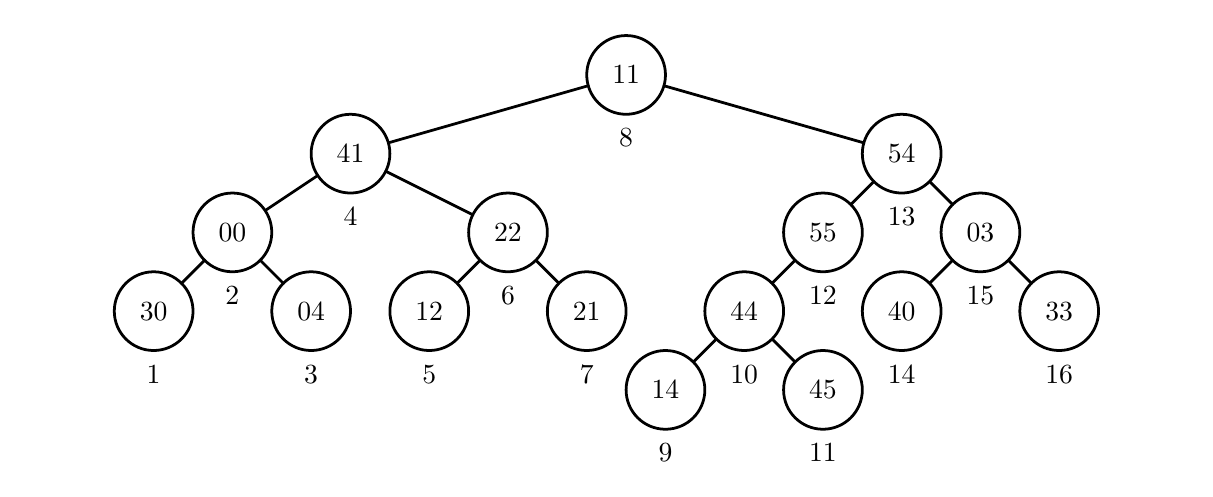
\begin{tikzpicture}[line cap=round,line join=round,x=1cm,y=1cm]
\clip(-.6,-1) rectangle (14.1,4.6);
\draw [line width=1pt] (1,1) circle (0.5cm);
\draw [line width=1pt] (2,2) circle (0.5cm);
\draw [line width=1pt] (3,1) circle (0.5cm);
\draw [line width=1pt] (5.5,2) circle (0.5cm);
\draw [line width=1pt] (6.5,1) circle (0.5cm);
\draw [line width=1pt] (3.5,3) circle (0.5cm);
\draw [line width=1pt] (7,4) circle (0.5cm);
\draw [line width=1pt] (10.5,3) circle (0.5cm);
\draw [line width=1pt] (9.5,2) circle (0.5cm);
\draw [line width=1pt] (8.5,1) circle (0.5cm);
\draw [line width=1pt] (11.5,2) circle (0.5cm);
\draw [line width=1pt] (10.5,1) circle (0.5cm);
\draw [line width=1pt] (12.5,1) circle (0.5cm);
\draw [line width=1pt] (4.5,1) circle (0.5cm);
\draw [line width=1pt] (7.5,0) circle (0.5cm);
\draw [line width=1pt] (9.5,0) circle (0.5cm);
\draw [line width=1pt] (1.3535533905932737,1.3535533905932737)-- (1.646446609406726,1.646446609406726);
\draw [line width=1pt] (2.353553390593274,1.646446609406726)-- (2.646446609406726,1.353553390593274);
i%\draw [line width=1pt] (2.646446609406726,0.646446609406726)-- (2.353553390593274,0.35355339059327395);
\draw [line width=1pt] (2.416025147168923,2.2773500981126156)-- (3.0839748528310773,2.722649901887385);
\draw [line width=1pt] (3.947213595499958,2.776393202250021)-- (5.052786404500042,2.223606797749979);
\draw [line width=1pt] (5.146446609406726,1.646446609406726)-- (4.853553390593274,1.353553390593274);
\draw [line width=1pt] (5.853553390593274,1.646446609406726)-- (6.146446609406726,1.353553390593274);
\draw [line width=1pt] (10.01923802617959,3.137360563948689)-- (7.480761973820412,3.8626394360513108);
\draw [line width=1pt] (6.519238026179588,3.8626394360513108)-- (3.9807619738204116,3.137360563948689);
\draw [line width=1pt] (10.146446609406727,2.646446609406727)-- (9.853553390593273,2.353553390593273);
\draw [line width=1pt] (9.146446609406727,1.646446609406727)-- (8.853553390593273,1.353553390593273);
\draw [line width=1pt] (8.146446609406727,0.6464466094067269)-- (7.853553390593274,0.35355339059327395);
\draw [line width=1pt] (8.853553390593273,0.6464466094067269)-- (9.146446609406727,0.35355339059327306);
\draw [line width=1pt] (10.853553390593273,1.353553390593273)-- (11.146446609406727,1.646446609406727);
\draw [line width=1pt] (11.146446609406727,2.353553390593273)-- (10.853553390593273,2.646446609406727);
\draw [line width=1pt] (11.853553390593273,1.646446609406727)-- (12.146446609406727,1.353553390593273);


\draw[color=black] (1,1) node {$30$};
\draw[color=black] (1,.2) node {1};
\draw[color=black] (2,2) node {$00$};
\draw[color=black] (2,1.2) node {2};
\draw[color=black] (3,1) node {$04$};
\draw[color=black] (3,.2) node {3};
\draw[color=black] (3.5,3) node {$41$};
\draw[color=black] (3.5,2.2) node {4};
\draw[color=black] (4.5,1) node {$12$};
\draw[color=black] (4.5,.2) node {5};
\draw[color=black] (5.5,2) node {$22$};
\draw[color=black] (5.5,1.2) node {6};
\draw[color=black] (6.5,1) node {$21$};
\draw[color=black] (6.5,.2) node {7};
\draw[color=black] (7,4) node {$11$};
\draw[color=black] (7,3.2) node {8};
\draw[color=black] (7.5,0) node {$14$};
\draw[color=black] (7.5,-.8) node {9};
\draw[color=black] (8.5,1) node {$44$};
\draw[color=black] (8.5,.2) node {10};
\draw[color=black] (9.5,0) node {$45$};
\draw[color=black] (9.5,-.8) node {11};
\draw[color=black] (9.5,2) node {$55$};
\draw[color=black] (9.5,1.2) node {12};
\draw[color=black] (10.5,3) node {$54$};
\draw[color=black] (10.5,2.2) node {13};
\draw[color=black] (10.5,1) node {$40$};
\draw[color=black] (10.5,.2) node {14};
\draw[color=black] (11.5,2) node {$03$};
\draw[color=black] (11.5,1.2) node {15};
\draw[color=black] (12.5,1) node {$33$};
\draw[color=black] (12.5,.2) node {16};


\end{tikzpicture}
}
\end{figure}
\begin{center}
{\large 11~12~22~21~11~14~44~45~55~54~44~40~00~04~44~43~33~34~44~41~11}

\end{center}
\end{frame}



\begin{frame}{Chaves implícitas}
\begin{figure}[htb]
\scalebox{.7}{
\centering
\begin{tikzpicture}[line cap=round,line join=round,>=triangle 45,x=1cm,y=1cm]
\clip(-.6,-1) rectangle (14.1,4.6);
\draw [line width=1pt] (1,1) circle (0.5cm);
\draw [line width=1pt] (2,2) circle (0.5cm);
\draw [line width=1pt] (3,1) circle (0.5cm);
\draw [line width=1pt] (5.5,2) circle (0.5cm);
\draw [line width=1pt] (6.5,1) circle (0.5cm);
\draw [line width=1pt] (3.5,3) circle (0.5cm);
\draw [line width=1pt] (7,4) circle (0.5cm);
\draw [line width=1pt] (10.5,3) circle (0.5cm);
\draw [line width=1pt] (9.5,2) circle (0.5cm);
\draw [line width=1pt] (8.5,1) circle (0.5cm);
\draw [line width=1pt] (11.5,2) circle (0.5cm);
\draw [line width=1pt] (10.5,1) circle (0.5cm);
\draw [line width=1pt] (12.5,1) circle (0.5cm);
\draw [line width=1pt] (4.5,1) circle (0.5cm);
\draw [line width=1pt] (7.5,0) circle (0.5cm);
\draw [line width=1pt] (9.5,0) circle (0.5cm);
\draw [line width=1pt] (1.3535533905932737,1.3535533905932737)-- (1.646446609406726,1.646446609406726);
\draw [line width=1pt] (2.353553390593274,1.646446609406726)-- (2.646446609406726,1.353553390593274);
i%\draw [line width=1pt] (2.646446609406726,0.646446609406726)-- (2.353553390593274,0.35355339059327395);
\draw [line width=1pt] (2.416025147168923,2.2773500981126156)-- (3.0839748528310773,2.722649901887385);
\draw [line width=1pt] (3.947213595499958,2.776393202250021)-- (5.052786404500042,2.223606797749979);
\draw [line width=1pt] (5.146446609406726,1.646446609406726)-- (4.853553390593274,1.353553390593274);
\draw [line width=1pt] (5.853553390593274,1.646446609406726)-- (6.146446609406726,1.353553390593274);
\draw [line width=1pt] (10.01923802617959,3.137360563948689)-- (7.480761973820412,3.8626394360513108);
\draw [line width=1pt] (6.519238026179588,3.8626394360513108)-- (3.9807619738204116,3.137360563948689);
\draw [line width=1pt] (10.146446609406727,2.646446609406727)-- (9.853553390593273,2.353553390593273);
\draw [line width=1pt] (9.146446609406727,1.646446609406727)-- (8.853553390593273,1.353553390593273);
\draw [line width=1pt] (8.146446609406727,0.6464466094067269)-- (7.853553390593274,0.35355339059327395);
\draw [line width=1pt] (8.853553390593273,0.6464466094067269)-- (9.146446609406727,0.35355339059327306);
\draw [line width=1pt] (10.853553390593273,1.353553390593273)-- (11.146446609406727,1.646446609406727);
\draw [line width=1pt] (11.146446609406727,2.353553390593273)-- (10.853553390593273,2.646446609406727);
\draw [line width=1pt] (11.853553390593273,1.646446609406727)-- (12.146446609406727,1.353553390593273);


\draw[color=black] (1,1) node {$30$};
\draw[color=black] (1,.2) node {1};
\draw[color=black] (2,2) node {$00$};
\draw[color=black] (2,1.2) node {3};
\draw[color=black] (3,1) node {$04$};
\draw[color=black] (3,.2) node {1};
\draw[color=black] (3.5,3) node {$41$};
\draw[color=black] (3.5,2.2) node {7};
\draw[color=black] (4.5,1) node {$12$};
\draw[color=black] (4.5,.2) node {1};
\draw[color=black] (5.5,2) node {$22$};
\draw[color=black] (5.5,1.2) node {3};
\draw[color=black] (6.5,1) node {$21$};
\draw[color=black] (6.5,.2) node {1};
\draw[color=black] (7,4) node {$11$};
\draw[color=black] (7,3.2) node {16};
\draw[color=black] (7.5,0) node {$14$};
\draw[color=black] (7.5,-.8) node {1};
\draw[color=black] (8.5,1) node {$44$};
\draw[color=black] (8.5,.2) node {3};
\draw[color=black] (9.5,0) node {$45$};
\draw[color=black] (9.5,-.8) node {1};
\draw[color=black] (9.5,2) node {$55$};
\draw[color=black] (9.5,1.2) node {4};
\draw[color=black] (10.5,3) node {$54$};
\draw[color=black] (10.5,2.2) node {8};
\draw[color=black] (10.5,1) node {$40$};
\draw[color=black] (10.5,.2) node {1};
\draw[color=black] (11.5,2) node {$03$};
\draw[color=black] (11.5,1.2) node {3};
\draw[color=black] (12.5,1) node {$33$};
\draw[color=black] (12.5,.2) node {1};


\end{tikzpicture}
}
\end{figure}
\begin{center}
{\large 11~12~22~21~11~14~44~45~55~54~44~40~00~04~44~43~33~34~44~41~11}
\end{center}
\end{frame}


\begin{frame}{Biblioteca de Euler Tour Trees}
\begin{exampleblock}{Biblioteca de Euler Tour Trees}
\begin{itemize}
\item  \treapCreate($u$,$v$): retorna uma ABB com um único nó com valor uv;
\item \treapJoin($T$,$R$): junta as ABBs $T$ e $R$ concatenando as sequências Eulerianas armazenada nelas e retorna a raiz da árvore resultante.
\item \treapSplit($T$, $\node$): corta~$T$ em duas ABBs. A primeira contendo todos os nós anteriores a~$\node$ e a segunda os demais;
\item \treapGetRoot($x$): retorna a raiz da ABB que contém $x$;
\item \treapSearch($T$,$k$): retorna o nó com chave $k$ da árvore $T$;
\item \treapOrder($\node$): retorna a chave de $\node$;
\item \treapGetLast($T$): retorna o nó de maior chave na árvore~$T$; e
\item \treapGetSize($T$): retorna o número de nós em $T$.
\end{itemize}
\end{exampleblock}
\boxpurple{\centering  \treapCreate{} e \treapGetSize{} :~$\O{1}$.\\ As demais operações :~$\O{\lg n}$.}
\end{frame}

\begin{frame}{Tabela de símbolos}
\boxblue{
\centering
Associa $(u,v) \rightarrow uv$.
}
\begin{exampleblock}{Biblioteca de tabela de símbolos}
\begin{itemize}
    \item $F \gets \hashCreate(n)$: cria e retorna um dicionário~$F$ para uma floresta dinâmica com~$n$ vértices;
    \item $F[u,v] \gets uv$: insere o nó que contém $uv$, com chave $(u,v)$ e valor associado~$uv$ na tabela~$F$.
    Se o par~$(u,v)$ já estiver presente no dicionário, então seu valor associado é substituído por~$uv$;
    \item $F[u,v] \gets \Nil{}$: remove o nó associado a~$(u,v)$ e seu valor associado do dicionário~$F$;
    \item $\var{} \gets F[u,v]$: atribui o valor associado à chave~$(u,v)$ à variável~\var;
	Caso a chave~$(u,v)$ não esteja presente em~$F$, atribui~$\Nil$ a~$\var{} $.
\end{itemize}
\end{exampleblock}
\boxpurple{
\centering
Consumo esperado~$\O{1}$ por rotina~\cite{CLRS}.
}
\end{frame}

\begin{frame}{Implementação da interface de floresta dinâmica}
\begin{algorithm}[H]
\caption{\dymForestCreate($n$)}
\label{Algo:dymForestCreate}
\begin{algorithmic}[1]
	\State \TODO{AAAAAAA}
\end{algorithmic}
\end{algorithm}
\boxpurple{
\centering
~~~~~\dymForestCreate{} : $\O{n}$\\
\dymForestQuery{}  : $\O{\lg n}$
}
\end{frame}

\begin{frame}{Implementação da interface de floresta dinâmica}
\begin{algorithm}[H]
\caption{\dymForestAddEdge($F$,$u$,$v$)}
\label{Algo:dymForestAddEdge}
\begin{algorithmic}[1]
\State \TODO{AAAAAAAAAAA}
\end{algorithmic}
\end{algorithm}
\boxpurple{
\centering
\dymForestAddEdge{}  : $\O{\lg n}$
}
\end{frame}

\begin{frame}{Rotina auxiliar \ETmovetofront{}}
\begin{algorithm}[H]
\caption{\ETmovetofront($F$,$u$)}
\label{Algo:ETmovetofront}
\begin{algorithmic}[1]
\State \TODO{AAAAAAAAAAA}
\end{algorithmic}
\end{algorithm}
\boxpurple{
\centering
\ETmovetofront{}  : $\O{\lg n}$
}
\end{frame}

\begin{frame}{Implementação da interface de floresta dinâmica}
\begin{algorithm}[H]
\caption{\dymForestDelEdge($F$, $u$, $v$)}
\label{Algo:dymForestDelEdge}
\begin{algorithmic}[1]
\State \TODO{AAAAAAAAAAA}
\end{algorithmic}
\end{algorithm}
\boxpurple{
\centering
\dymForestDelEdge{}  : $\O{\lg n}$
}
\end{frame}

\subsection{Treaps}
\begin{frame}{Uma treap imersa no plano cartesiano.}
\boxblue{
\centering
Cada nó da treap possui um par ordenado \textbf{(chave,prioridade)}
}
\begin{figure}[htb]
\centering
\scalebox{.45}{
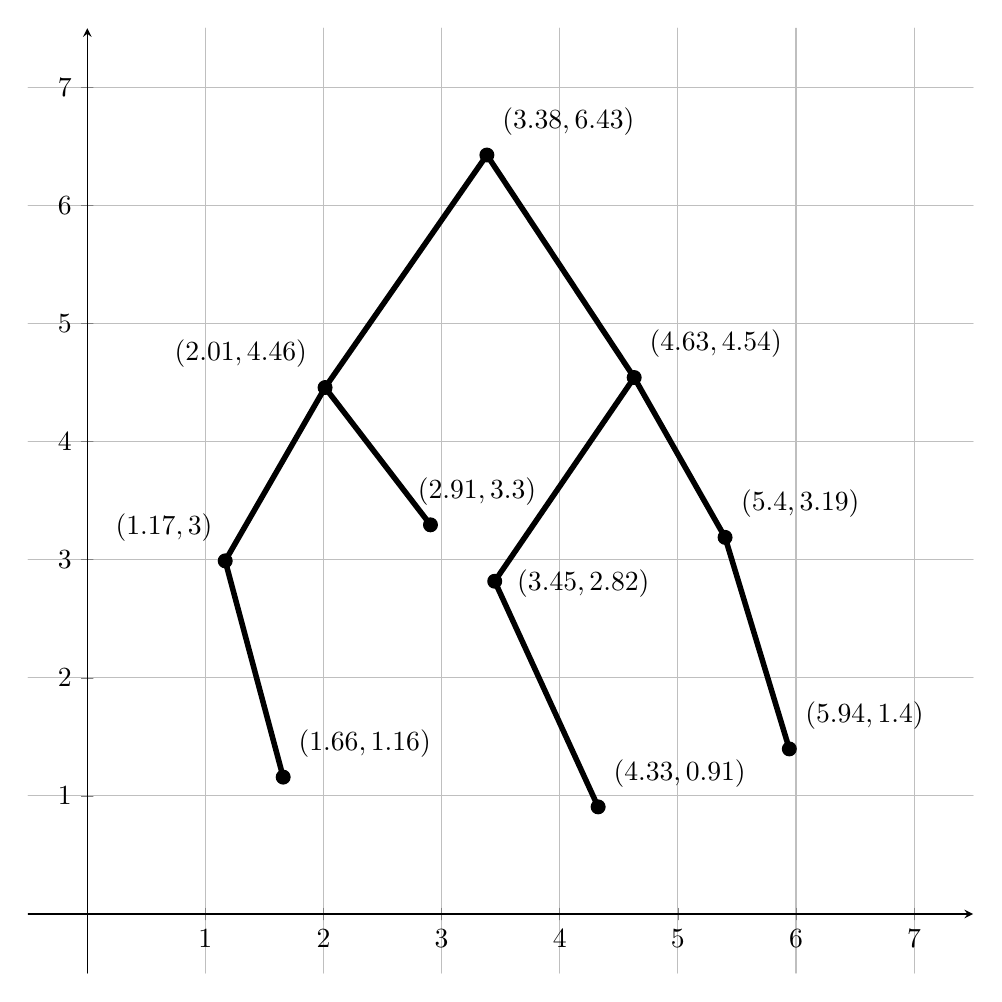
\begin{tikzpicture}[line cap=round,line join=round,x=1cm,y=1cm]
\begin{axis}[
x=1.5cm,y=1.5cm,
axis lines=middle,
ymajorgrids=true,
xmajorgrids=true,
xmin=-.5,
xmax=7.5,
ymin=-.5,
ymax=7.5,
xtick={-3,-2,...,16},
ytick={-1,0,...,10},]
\clip(-1,-1) rectangle (16.11970291004026,10.724908935002318);
\draw [line width=2pt] (3.383319601128083,6.426379568244459)-- (2.0132670659467835,4.457693392208796);
\draw [line width=2pt] (3.383319601128083,6.426379568244459)-- (4.630423800125734,4.5424562038011995);
\draw [line width=2pt] (2.0132670659467835,4.457693392208796)-- (1.1677195880152356,2.990209488027528);
\draw [line width=2pt] (2.0132670659467835,4.457693392208796)-- (2.9057052270438763,3.295352004803549);
\draw [line width=2pt] (4.630423800125734,4.5424562038011995)-- (3.449654930862001,2.8177376307193422);
\draw [line width=2pt] (4.630423800125734,4.5424562038011995)-- (5.399913625039178,3.189215477229281);
\draw [line width=2pt] (3.449654930862001,2.8177376307193422)-- (4.325281283349713,0.9072801343825158);
\draw [line width=2pt] (5.399913625039178,3.189215477229281)-- (5.943863328857303,1.3981615744135059);
\draw [line width=2pt] (1.1677195880152356,2.990209488027528)-- (1.6586010280462258,1.1593543873714025);
\begin{scriptsize}
\draw [fill=black] (3.383319601128083,6.426379568244459) circle (2.5pt);
\draw[color=black] (4.073207030360826,6.711621486100305) node {$(3.38, 6.43)$};
\draw [fill=black] (2.0132670659467835,4.457693392208796) circle (2.5pt);
\draw[color=black] (1.3,4.748095725976344) node {$(2.01, 4.46)$};
\draw [fill=black] (4.630423800125734,4.5424562038011995) circle (2.5pt);
\draw[color=black] (5.320311229358477,4.827698121657045) node {$(4.63, 4.54)$};
\draw [fill=black] (1.1677195880152356,2.990209488027528) circle (2.5pt);
\draw[color=black] (.65,3.275451405883374) node {$(1.17, 3)$};
\draw [fill=black] (2.9057052270438763,3.295352004803549) circle (2.5pt);
\draw[color=black] (3.3,3.5805939226593946) node {$(2.91, 3.3)$};
\draw [fill=black] (3.449654930862001,2.8177376307193422) circle (2.5pt);
\draw[color=black] (4.2,2.8) node {$(3.45, 2.82)$};
\draw [fill=black] (5.399913625039178,3.189215477229281) circle (2.5pt);
\draw[color=black] (6.036732790484788,3.4744573950851265) node {$(5.4, 3.19)$};
\draw [fill=black] (4.325281283349713,0.9072801343825158) circle (2.5pt);
\draw[color=black] (5.015168712582456,1.1925220522383615) node {$(4.33, 0.91)$};
\draw [fill=black] (5.943863328857303,1.3981615744135059) circle (2.5pt);
\draw[color=black] (6.580682494302912,1.6834034922693517) node {$(5.94, 1.4)$};
\draw [fill=black] (1.6586010280462258,1.1593543873714025) circle (2.5pt);
\draw[color=black] (2.3484884572789686,1.4445963052272481) node {$(1.66, 1.16)$};
\end{scriptsize}
\end{axis}
\end{tikzpicture}}
\end{figure}
\end{frame}

\section{Conexidade em grafos dinâmicos}
\begin{frame}{Conexidade em grafos dinâmicos}
\begin{exampleblock}{Conexidade em grafos dinâmicos}
\begin{itemize}
\item \dymGraphCreate($n$): cria um grafo dinâmico com $n$ vértices isolados;
\item \dymGraphAddEdge($G$,$u$,$v$): adiciona a aresta $uv$ ao grafo dinâmico $G$;
\item \dymGraphDelEdge($G$,$u$,$v$): remove a aresta $uv$ de $G$; e
\item \dymGraphQuery($G$,$u$,$v$): retorna verdadeiro se $u$ e $v$ estão na mesma componente conexa de $G$ e falso, caso contrário.
\end{itemize}
\end{exampleblock}

\end{frame}

\begin{frame}{Ideia inicial}
\begin{block}{Manteremos}
\begin{itemize}
    \item floresta maximal dinâmica~$F$ de~$G$; e
    \item um grafo~$R$ = $G-F$
\end{itemize}
\end{block}

\begin{exampleblock}{Lista de adjacências}
\begin{itemize}
    \item \graphCreate($n$): devolve a representação por listas de adjacências de um grafo com~$n$ vértices isolados.
    \item \graphAdd($G$,$u$,$v$): adiciona $u$ na lista de adjacências de $v$ em $G$ e vice-versa.
    \item \graphDel($G$,$u$,$v$): remove $u$ da lista de adjacências de $v$ em $G$ e vice-versa.
\end{itemize}
\end{exampleblock}
\boxpurple{
\centering
~~~~~~\graphCreate{} : $\O{n}$\\
\graphAdd{}  : $\O{1}$\\
\graphDel{}  : $\O{1}$\\
}
\end{frame}


\begin{frame}{Ideia inicial}
\begin{algorithm}[H]
\caption{\dymGraphQuery($G$, $u$, $v$)}
\label{Algo:dymGraphQuery}
\begin{algorithmic}[1]
\State $i$ 
\end{algorithmic}
\end{algorithm}
\boxpurple{
\dymGraphQuery{} : $\O{\lg n}$\\
\dymGraphAddEdge{}  : $\O{\lg^2 n}$ amortizado\TODO{!!}
}
\end{frame}



\begin{frame}{Remoção de arestas}
\begin{block}{Estrutura de níveis}
\begin{itemize}
    \item Cada aresta possui um \defi{nível}, que é um inteiro entre~$1$ e $\lceil \log n \rceil$;
    \item Arestas serão inseridas no nível~$\lceil \log n \rceil$;
    \item O nível de uma aresta pode diminuir, mas nunca aumentar. 
\end{itemize}
\end{block}
\begin{block}{Estrutura}
$G_i$: grafo com arestas de nível $\leqslant i$. Para cada camada $i$, manteremos:
\begin{itemize}
    \item $F_i$: floresta maximal  de~$G_i$; e
    \item $R_i$: arestas de nível~$i \notin F_i$.
\end{itemize}
\end{block}
\begin{block}{Invariantes}
\begin{itemize}
    \item $F_i \subseteq F_{i+1}$, para cada $1\leqslant i \leqslant \lceil \log n \rceil-1$ e que $F_i$ é uma floresta maximal de~$G_i$; e
    \item Cada componente de $F_i$ possui menos do que $2^i$ arestas.
\end{itemize}
\end{block}
\end{frame}

\begin{frame}{Implementações}
\begin{exampleblock}{Adaptações}
\centering
$G.F\rightarrow G.F_{\lceil \log n \rceil}$\\
$G.R\rightarrow G.R_{\lceil \log n \rceil}$
\end{exampleblock}
\begin{algorithm}[H]
\caption{\dymGraphDelEdge($G$, $u$, $v$)}
\label{Algo:dymGraphDelEdge}
\begin{algorithmic}[1]
\If {$uv \in G.F_{\lceil \lg n \rceil}$}
  \For {$i \gets uv.nível$ até $\lceil \lg n \rceil$}
    \State \dymForestDelEdge($G$.$F$[i],$u$,$v$))
  \EndFor
  \State \dymGraphReplace($G$,$u$,$v$,$uv$.$nível$)
\Else
  \State \graphDel($G$.$R$[$uv$.$nível$],$u$,$v$)
\EndIf
\end{algorithmic}
\end{algorithm}
\boxpurple{
\centering
\dymGraphDelEdge{}  : $\O{\lg^2 n}$ amortizado.
}
\end{frame}

\begin{frame}{Estrutura de níveis}
\begin{figure}[htb]
\scalebox{.5}{
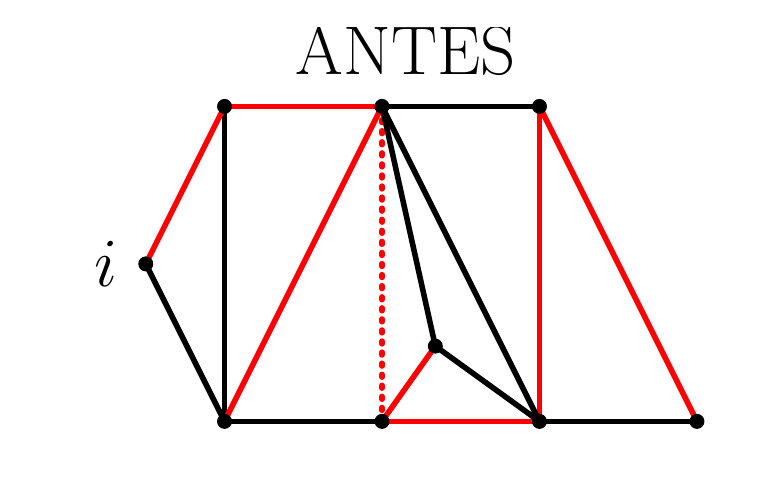
\begin{tikzpicture}[line cap=round,line join=round,x=1cm,y=1cm]
\clip(-1.5,-.5) rectangle (7.5,5);
\draw (3.3,4.7) node {{\Huge ANTES}};
\draw (-.5,2) node {{\Huge $i$}};
\draw [line width=2pt,color=ccqqqq] (3,0)-- (3.677138935355088,0.9555967043150745);
\draw [line width=2pt] (3,0)-- (1,0);
\draw [line width=2pt] (1,0)-- (1,4);
\draw [line width=2pt] (1,0)-- (0,2);
\draw [line width=2pt,color=ccqqqq,dash pattern=on 1pt off 3pt] (3,0)-- (3,4);
\draw [line width=2pt,color=ccqqqq] (3,0)-- (5,0);
\draw [line width=2pt,color=ccqqqq] (5,0)-- (5,4);
\draw [line width=2pt,color=ccqqqq] (1,4)-- (3,4);
\draw [line width=2pt] (3,4)-- (5,0);
\draw [line width=2pt] (3.677138935355088,0.9555967043150745)-- (5,0);
\draw [line width=2pt] (5,4)-- (3,4);
\draw [line width=2pt,color=ccqqqq] (1,4)-- (0,2);
\draw [line width=2pt,color=ccqqqq] (1,0)-- (3,4);
\draw [line width=2pt] (3,4)-- (3.677138935355088,0.9555967043150745);
\draw [line width=2pt,color=ccqqqq] (5,4)-- (7,0);
\draw [line width=2pt] (7,0)-- (5,0);
\begin{scriptsize}
\draw [fill=black] (3,0) circle (2.5pt);
\draw [fill=black] (3.677138935355088,0.9555967043150745) circle (2.5pt);
\draw [fill=black] (1,0) circle (2.5pt);
\draw [fill=black] (1,4) circle (2.5pt);
\draw [fill=black] (0,2) circle (2.5pt);
\draw [fill=black] (3,4) circle (2.5pt);
\draw [fill=black] (5,0) circle (2.5pt);
\draw [fill=black] (5,4) circle (2.5pt);
\draw [fill=black] (7,0) circle (2.5pt);
\end{scriptsize}
\end{tikzpicture}

\begin{tikzpicture}[line cap=round,line join=round,x=1cm,y=1cm]
\clip(0,-.5) rectangle (5,4.5);
\end{tikzpicture}
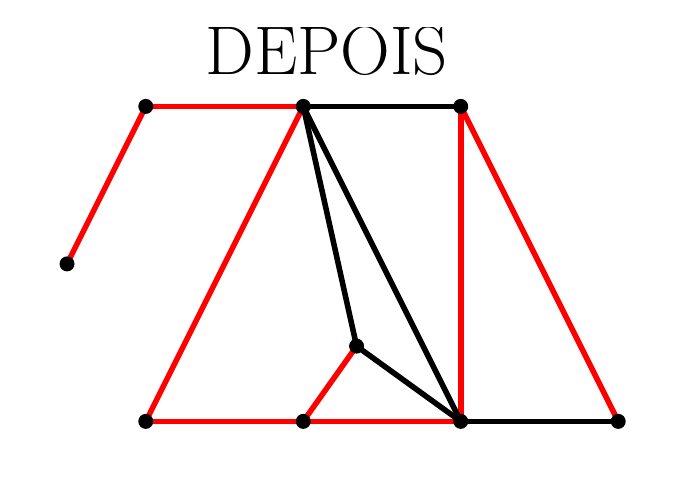
\begin{tikzpicture}[line cap=round,line join=round,x=1cm,y=1cm]
\clip(-.5,-.5) rectangle (7.5,5);
\draw (3.3,4.7) node {{\Huge DEPOIS}};
\draw [line width=2pt,color=ccqqqq] (3,0)-- (3.677138935355088,0.9555967043150745);
\draw [line width=2pt,color=ccqqqq] (3,0)-- (1,0);
\draw [line width=2pt,color=ccqqqq] (3,0)-- (5,0);
\draw [line width=2pt,color=ccqqqq] (5,0)-- (5,4);
\draw [line width=2pt,color=ccqqqq] (1,4)-- (3,4);
\draw [line width=2pt] (3,4)-- (5,0);
\draw [line width=2pt] (3.677138935355088,0.9555967043150745)-- (5,0);
\draw [line width=2pt] (5,4)-- (3,4);
\draw [line width=2pt,color=ccqqqq] (1,4)-- (0,2);
\draw [line width=2pt,color=ccqqqq] (1,0)-- (3,4);
\draw [line width=2pt] (3,4)-- (3.677138935355088,0.9555967043150745);
\draw [line width=2pt,color=ccqqqq] (5,4)-- (7,0);
\draw [line width=2pt] (7,0)-- (5,0);
\begin{scriptsize}
\draw [fill=black] (3,0) circle (2.5pt);
\draw [fill=black] (3.677138935355088,0.9555967043150745) circle (2.5pt);
\draw [fill=black] (1,0) circle (2.5pt);
\draw [fill=black] (1,4) circle (2.5pt);
\draw [fill=black] (0,2) circle (2.5pt);
\draw [fill=black] (3,4) circle (2.5pt);
\draw [fill=black] (5,0) circle (2.5pt);
\draw [fill=black] (5,4) circle (2.5pt);
\draw [fill=black] (7,0) circle (2.5pt);
\end{scriptsize}
\end{tikzpicture}
}
\end{figure}
\begin{figure}[htb]
\scalebox{.5}{
\begin{tikzpicture}[line cap=round,line join=round,x=1cm,y=1cm]
\clip(-2,-.5) rectangle (7.5,4.5);
\draw (-1,2) node {{\Huge $i-1$}};
\begin{scriptsize}
\draw [fill=black] (3,0) circle (2.5pt);
\draw [fill=black] (3.677138935355088,0.9555967043150745) circle (2.5pt);
\draw [fill=black] (1,0) circle (2.5pt);
\draw [fill=black] (1,4) circle (2.5pt);
\draw [fill=black] (0,2) circle (2.5pt);
\draw [fill=black] (3,4) circle (2.5pt);
\draw [fill=black] (5,0) circle (2.5pt);
\draw [fill=black] (5,4) circle (2.5pt);
\draw [fill=black] (7,0) circle (2.5pt);
\end{scriptsize}
\end{tikzpicture}

\begin{tikzpicture}[line cap=round,line join=round,x=1cm,y=1cm]
\clip(0,-.5) rectangle (5,4.5);
\end{tikzpicture}
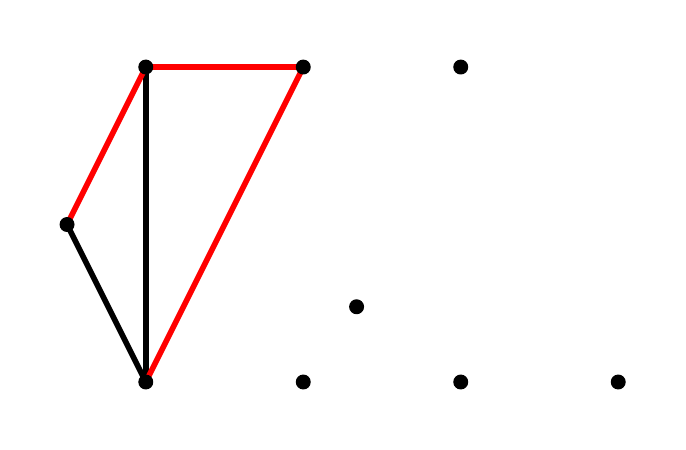
\begin{tikzpicture}[line cap=round,line join=round,x=1cm,y=1cm]
\clip(-.5,-.5) rectangle (7.5,4.5);
\draw [line width=2pt] (1,0)-- (1,4);
\draw [line width=2pt] (1,0)-- (0,2);
\draw [line width=2pt,color=ccqqqq] (1,4)-- (3,4);
\draw [line width=2pt,color=ccqqqq] (1,4)-- (0,2);
\draw [line width=2pt,color=ccqqqq] (1,0)-- (3,4);
\begin{scriptsize}
\draw [fill=black] (3,0) circle (2.5pt);
\draw [fill=black] (3.677138935355088,0.9555967043150745) circle (2.5pt);
\draw [fill=black] (1,0) circle (2.5pt);
\draw [fill=black] (1,4) circle (2.5pt);
\draw [fill=black] (0,2) circle (2.5pt);
\draw [fill=black] (3,4) circle (2.5pt);
\draw [fill=black] (5,0) circle (2.5pt);
\draw [fill=black] (5,4) circle (2.5pt);
\draw [fill=black] (7,0) circle (2.5pt);
\end{scriptsize}
\end{tikzpicture}}
\end{figure}
\end{frame}




\begin{frame}{A rotina \dymGraphReplace{}}
\begin{algorithm}[H]
\caption{\dymGraphReplace($G$,$u$,$v$,$nível$)}
\label{Algo:dymGraphReplace}
\begin{algorithmic}[1]
\State $i$
\end{algorithmic}
\end{algorithm}
\end{frame}


\section{Floresta maximal de peso mínimo em grafos planos}

\begin{frame}{Floresta maximal de peso mínimo}
\begin{exampleblock}{O problema da floresta maximal de peso mínimo em grafos planos}
\begin{itemize}
\item \MSFCreate($n$): devolve um grafo dinâmico com $n$ vértices isolados;
\item \MSFaddEdge($G$,$u$,$v$,$w$): adiciona $uv$ com peso $w$ a~$G$;
\item \MSFdelEdge($G$,$u$,$v$): remove $uv$ de~$G$; e
\item \MSFweight($G$): devolve o peso de uma MSF de $G$.
\end{itemize}
\end{exampleblock}

\end{frame}


\begin{frame}{Caso decremental}
\begin{exampleblock}{O caso decremental do problema MSF em grafos ponderados dinâmicos}
\begin{itemize}
\item \MSFCreate($H$): recebe um grafo~$H$ e devolve um grafo dinâmico e uma MSF dele;
\item \MSFdelEdge($G$,$u$,$v$): remove $uv$ de~$G$; e
\item \MSFweight($G$): devolve o peso de uma MSF de $G$.
\end{itemize}
\end{exampleblock}
\begin{exampleblock}{Adaptação para o caso decremental}
\begin{itemize}
    \item $F_{\lceil \log n \rceil}$ deve ser de peso mínimo;
    \item Em \dymGraphReplace{}, percorrer as arestas de nível $i$ em ordem crescente de peso;
\end{itemize}
\end{exampleblock}
\end{frame}







\section{Bibliografia}
\begin{frame}[allowframebreaks]
\frametitle{Bibliografia}
\bibliographystyle{plain}
    \bibliography{bib.bib}
\end{frame}

\end{document}
